\documentclass[noinstructornotes]{ximera}
%handout:  for handout version with no solutions or instructor notes
%handout,instructornotes:  for instructor version with just problems and notes, no solutions
%noinstructornotes:  shows only problem and solutions

%% handout
%% space
%% newpage
%% numbers
%% nooutcomes

%I added the commands here so that I would't have to keep looking them up
%\newcommand{\RR}{\mathbb R}
%\renewcommand{\d}{\,d}
%\newcommand{\dd}[2][]{\frac{d #1}{d #2}}
%\renewcommand{\l}{\ell}
%\newcommand{\ddx}{\frac{d}{dx}}
%\everymath{\displaystyle}
%\newcommand{\dfn}{\textbf}
%\newcommand{\eval}[1]{\bigg[ #1 \bigg]}

%\begin{image}
%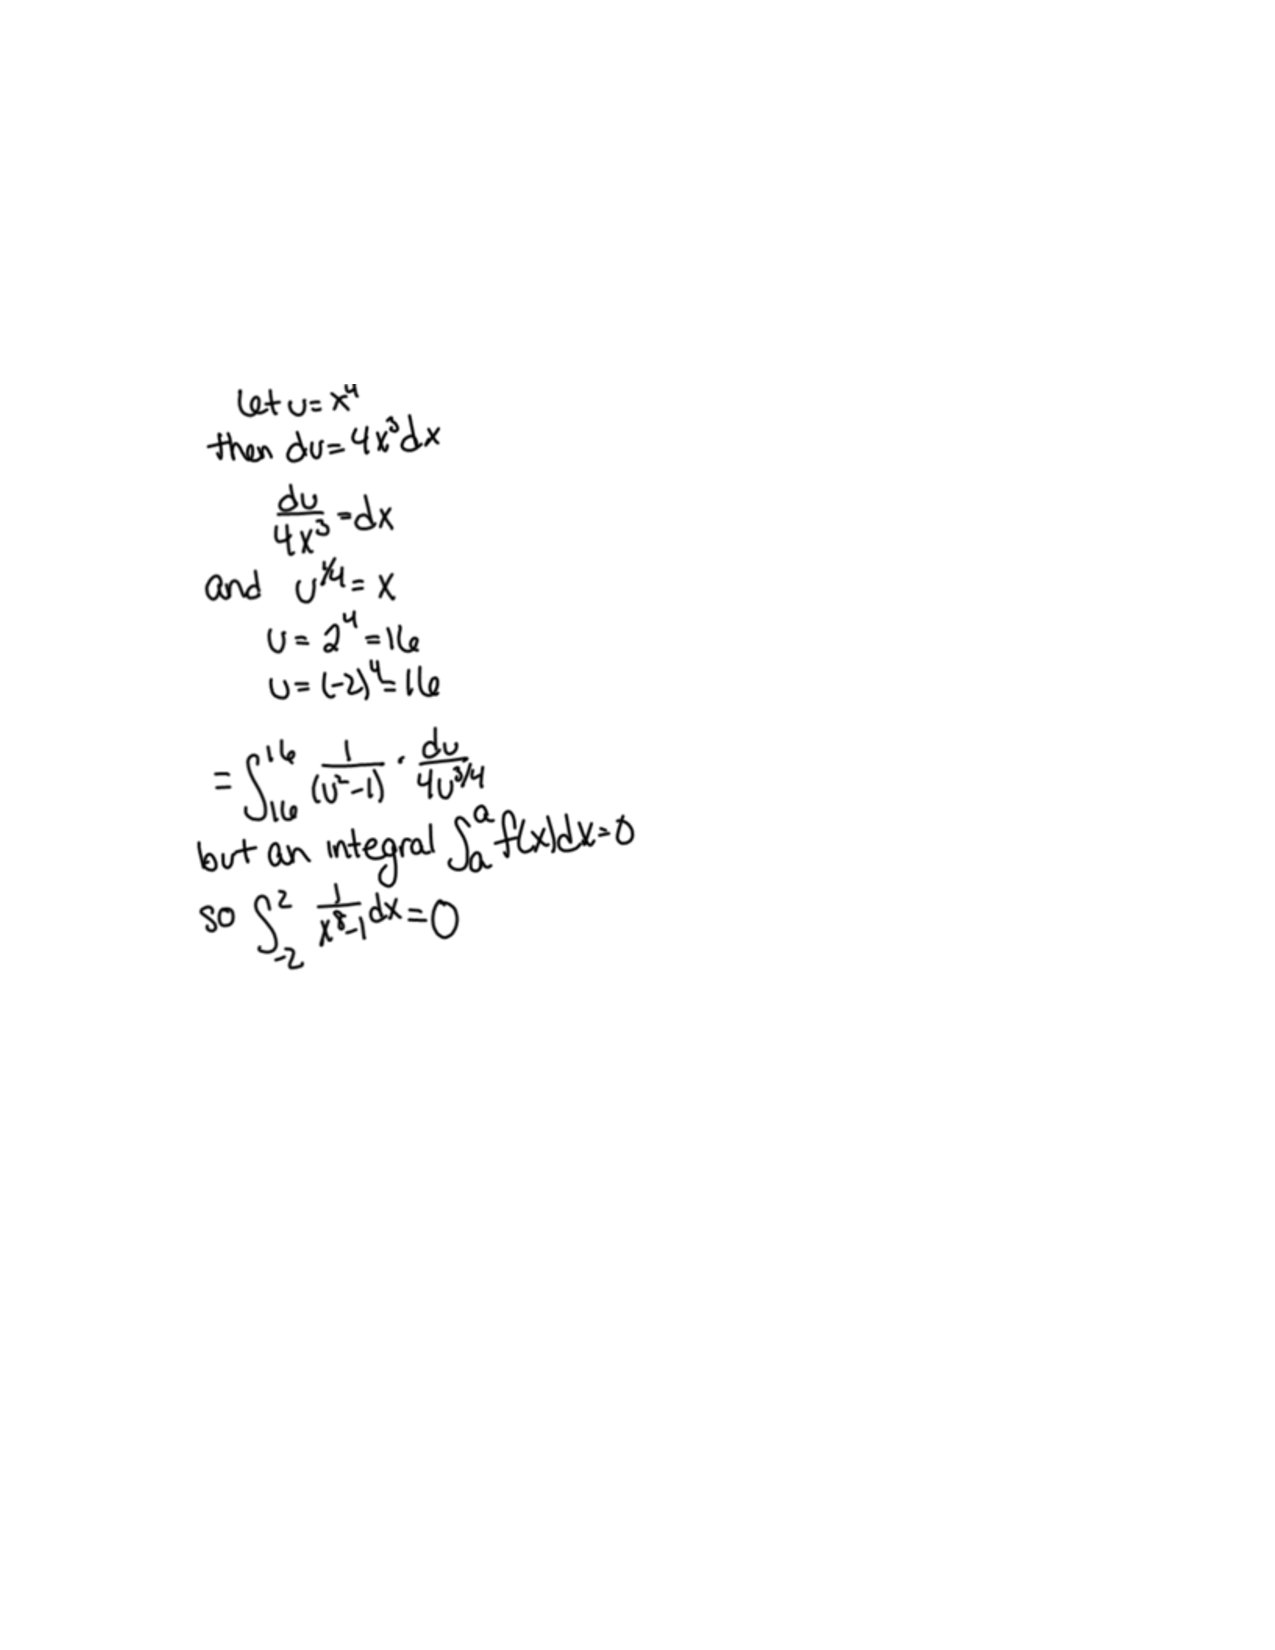
\includegraphics[trim= 170 420 250 180]{Figure1.pdf}
%\end{image}

%add a ``.'' below when used in a specific directory.
\newcommand{\RR}{\mathbb R}
\renewcommand{\d}{\,d}
\newcommand{\dd}[2][]{\frac{d #1}{d #2}}
\renewcommand{\l}{\ell}
\newcommand{\ddx}{\frac{d}{dx}}
\newcommand{\dfn}{\textbf}
\newcommand{\eval}[1]{\bigg[ #1 \bigg]}

\usepackage{multicol}

\renewenvironment{freeResponse}{
\ifhandout\setbox0\vbox\bgroup\else
\begin{trivlist}\item[\hskip \labelsep\bfseries Solution:\hspace{2ex}]
\fi}
{\ifhandout\egroup\else
\end{trivlist}
\fi} %% we can turn off input when making a master document


\title{Sections 6.8 and 6.9: Exponential Models}  

\begin{document}
\begin{abstract}		\end{abstract}
\maketitle



\begin{comment}
\section{Warm up:}

	\begin{freeResponse}
	
	\end{freeResponse}
	
\begin{instructorNotes}

\end{instructorNotes}
\end{comment}







\section{Group work:}



%problem 1
\begin{problem}
Vitameatavegamin is a strange substance that comes in two forms.  
V-I decays at a linear rate, while V-II decays at an exponential rate.  
Both have the property that $10$ ounces will decrease to $7$ ounces in $6$ hours.  
For each of V-I and V-II, answer the following:
	\begin{enumerate}
	
	\item  If we started with $80$ ounces, how much will there be $6$ hours later?
	\begin{freeResponse}
	\dfn{V-I:}  Recall that in the linear decay model
		\[
		y(t) = -k \cdot t + y_0
		\]
	where $k$ denotes the rate of decay and $y_0$ is the initial amount.  
	We are given that $y_0 = 80oz$.  
	Clearly, we also have that
		\[
		y'(t) = -k.
		\]
	In the linear decay model, the rate of decay does not depend on the initial amount.  
	So from the given information, we have that
		\[
		-k = \frac{10oz - 7oz}{0hr - 6hr} = - \frac{1}{2}.  
		\]
	Thus, $y(t) = - \frac{1}{2} t + 80$, and therefore
		\[
		y(6) = - \frac{1}{2} (6) + 80 = 77 oz.
		\]
		
	\vskip 10pt	
		
	\dfn{V-II:}  Recall that in the exponential decay model
		\[
		y(t) = y_0 \cdot e^{-k \cdot t}
		\]
	where again $y_0 = 80oz$ is the initial amount.  
	Also notice that
		\begin{align*}
		y'(t) &= -k y_0 e^{-kt}  \\
		&= -k y(t)  \\
		\Longrightarrow &\qquad y'(0) = -k y_0.
		\end{align*}
	
	It is given that it takes $6$ hours for $10$ ounces to decrease to $7$ ounces.  
	In other words, it takes $6$ hours for $70\%$ of the substance to remain.
	So we have that
		\begin{align*}
		y(6) &= \frac{7}{10} y_0  \\
		&\Longrightarrow  \qquad  y_0 e^{-k \cdot 6} = \frac{7}{10} y_0  \\
		&\Longrightarrow  \qquad  e^{-6k} = \frac{7}{10}  \\
		&\Longrightarrow  \qquad -6k = \ln \left(\frac{7}{10} \right) = - \ln \left( \frac{10}{7} \right)  \\
		&\Longrightarrow  \qquad  k = \frac{1}{6} \ln \left( \frac{10}{7} \right).
		\end{align*}
	Thus,
		\begin{align*}
		y(6) &= 80 e^{- \frac{1}{6} \ln \left( \frac{10}{7} \right) \cdot 6}  \\
		&= 80 e^{- \ln \left( \frac{10}{7} \right)}  \\
		&= 80 \cdot \frac{7}{10} = 56oz.
		\end{align*}
	\end{freeResponse}
	
	
	
	\item  How long will it take to decrease from $15$ ounces to $7.5$ ounces?
	\begin{freeResponse}
	\dfn{V-I:}  Recall from above that $k = \frac{1}{2}$.  
	Then since $y_0$ is now $15$, we have that
		\[
		y(t) = - \frac{1}{2} t + 15.
		\]
	We want to find $t$ such that $y(t) = 7.5$.  
	So we solve
		\begin{align*}
		7.5 &= - \frac{1}{2} t + 15  \\
		- \frac{15}{2} &= - \frac{1}{2} t  \\
		t &= 15 \text{ hours}.
		\end{align*}
		
	\vskip 10pt
	
	\dfn{V-II:}  Again, since $y_0$ is now $15$, we know from above that
		\[
		y(t) = 15 e^{- \frac{1}{6} \ln \left( \frac{10}{7} \right) \cdot t}.
		\]
	We want to find $t$ such that $y(t) = 7.5 = \frac{15}{2}$.  So we solve
		\begin{align*}
		\frac{15}{2} &= 15 e^{- \frac{1}{6} \ln \left( \frac{10}{7} \right) \cdot t}  \\
		\frac{1}{2} &= e^{- \frac{1}{6} \ln \left( \frac{10}{7} \right) \cdot t}  \\
		\ln \left( \frac{1}{2} \right) &= - \frac{1}{6} \ln \left( \frac{10}{7} \right) \cdot t  \\
		\ln \left( \frac{10}{7} \right) t &= - 6 \ln \left( \frac{1}{2} \right) = 6 \ln 2  \\
		t &= \frac{6 \ln 2}{\ln \left( \frac{10}{7} \right) } \text{ hours}.
		\end{align*}
	\end{freeResponse}
	
	\end{enumerate}
	
\end{problem}

\begin{instructorNotes}
The issue is to compare and contrast linear and exponential decay.  
To solve, it is implicit to find the slope (I) and $k$ (II) first before proceeding (this may need a prompt).
\end{instructorNotes}














								
				
				
	














\end{document} 


















